%\documentclass[a4paper,12pt,final,twoside]{scrartcl}
\setcounter{secnumdepth}{3}
\setcounter{tocdepth}{5}

\usepackage[utf8]{inputenc}
\usepackage[T1]{fontenc}
\linespread{1.4}
\usepackage{dsfont}
\usepackage{amsfonts}
\usepackage{amsmath}
\usepackage{amssymb}
\usepackage{amsthm}
\usepackage{mathtools}
\usepackage{mathbbol}
\usepackage{amsmath1}
\usepackage[ngerman]{babel}
\usepackage{bibgerm}
\usepackage[pdftex]{graphicx}
%\usepackage{mathpazo}
\usepackage{floatflt}
%%\usepackage{epsfig}
\usepackage{wrapfig}
\usepackage{graphicx}
\usepackage{tabularx}
\usepackage{caption} 
\usepackage{multicol} 
\usepackage{mathrsfs}
%\usepackage{pspicture}
%\usepackage{eepic}
%\usepackage{epic}
%\usepackage{trfsigns}

%\usepackage[ansinew]{inputenc}
\usepackage{longtable,array,dcolumn}
%\usepackage{ngerman}
\usepackage{epic}
\usepackage{rotate}
\usepackage{graphpap}
\usepackage{amssymb}
\usepackage[squaren]{SIunits}
\usepackage{curves}
\usepackage{float}
\usepackage{array}
\usepackage{enumerate}
\usepackage{marvosym}
\usepackage{slashed}%für feynmanslsash
\usepackage[breaklinks,pdfborder={0 0 0}]{hyperref}
\usepackage{ulem}	%angeblich funktioniert dann
\let\underbar\uline	%underbar in math auch bei greek letters
\usepackage{multirow}
%\usepackage{multicolumn}
\usepackage{enumitem}


\setlength{\parskip}{12pt}
\setlength{\parindent}{0mm}
%\newcommand{\grad}{\ensuremath{^{\circ}}
%\renewcommand{\figurename}{Abb.}		% mit usepackage caption2
%\renewcommand{\captionfont}{\small \itshape}	% mit usepackage caption2
%\setkomafont{caption}{\small \itshape}		%sollte mit caption im userpackage funktionieren
%\setkomafont{captionlabel}{\small , \itshape}	%sollte mit caption im userpackage funktionieren
\captionsetup{font = {small, sf}} %mit it anstelle von sf gibts kusiv

\date{2009-20-10}
\newcommand{\kreis}[1]{
 \qbezier(-#1,0)(-#1,#1)(0,#1)
  \qbezier(0,#1)(#1,#1)(#1,0)
  \qbezier(#1,0)(#1,-#1)(0,-#1)
  \qbezier(0,-#1)(-#1,-#1)(-#1,0)}
\newcommand{\s}{\ \big| \ }
\newcommand{\lo}{\left <}
\newcommand{\ro}{\ri >}
\newcommand{\g}{&=&}

\newcommand{\ham}{\mathcal H}
\newcommand{\hil}{\mathscr H}
\newcommand{\fok}{\mathscr F}
\newcommand{\wh}{\widehat}
%\newcommand{\left}{\left}
\newcommand{\ri}{\right}
\newcommand{\Sp}{\text{Sp}}
\newcommand{\babsatz}{\par \begingroup \leftskip=2cm}
\newcommand{\eabsatz}{\par\endgroup}

\newcommand{\D}{\text{\itshape D}}
\newcommand{\Lr}{\mathcal L }%\textit{L}}
\newcommand{\rot}{\text{rot}}
\newcommand{\divergenz}{\text{div}}
\newcommand{\grad}{\text{grad}}
\newcommand{\grat}{${}^{\circ}$}
%\newcommand{\tanh}{\text{tanh}} already defined

\newcommand{\RM}[1]{\text{\MakeUppercase{\romannumeral #1}}}
\newcommand{\dell}{\partial}
\renewcommand{\div}{\operatorname{div}}
\newcommand{\I}{\dot{\text{\i\!\i}}}
\newcommand{\e}{\mathrm{e}}
\newcommand{\ket}[1]{\mid\!\!\!\,\,{#1}\rangle}
\newcommand{\bra}[1]{\langle{#1}\!\!\!\,\,\mid}
\newcommand{\braket}[2]{\langle{#1}\!\!\!\,\,\mid\!\!\!\,\,{#2}\rangle}
\newcommand{\bracket}[3]{\langle{#1}\!\!\!\,\,\mid\!\!\!\,\,{#2}\!\!\!\,\,\mid\!\!\!\,\,{#3}\rangle}
\newcommand{\1}{\mathds{1}}
\newcommand{\EW}[1]{\langle\!\!\,\,#1\!\!\,\,\rangle}
\newcommand{\arrowbox}[1]{-\!\!\!\!\:\text{(#1)}\!\!\!\;\;\!\!\!\rightarrow}

\newcommand{\ketI}[1]{\ket{#1}_{\!\!\;\text{I}}}
\newcommand{\ketII}[1]{\ket{#1}_{\!\!\;\text{II}}}
\newcommand{\ketIII}[1]{\ket{#1}_{\!\!\;\text{III}}}
\newcommand{\braI}[1]{\,\!_{\text{I}\!\!\;}\bra{#1}}
\newcommand{\braII}[1]{\,\!_{\text{II}\!\!\;}\bra{#1}}
\newcommand{\braketI}[2]{\,_{\text{I}\!\!\;}\braket{#1}{#2}_{\!\!\;\text{I}}\,}
\newcommand{\braketII}[2]{\,_{\text{II}\!\!\;}\braket{#1}{#2}_{\!\!\;\text{II}}\,}
\newcommand{\braketIII}[2]{\,_{\text{III}\!\!\;}\braket{#1}{#2}_{\!\!\;\text{III}}\,}
\newcommand{\bracketI}[3]{\,_{\text{I}\!\!\;}\bracket{#1}{#2}{#3}_{\!\!\;\text{I}}\,}
\newcommand{\bracketII}[3]{\,_{\text{II}\!\!\;}\bracket{#1}{#2}{#3}_{\!\!\;\text{II}}\,}


\newcommand{\up}{\ket{\uparrow}}
\newcommand{\updg}{\bra{\uparrow}}
\newcommand{\down}{\ket{\downarrow}}
\newcommand{\downdg}{\bra{\downarrow}}
\newcommand{\upup}{\ket{\uparrow\uparrow}}
\newcommand{\updown}{\ket{\uparrow\downarrow}}
\newcommand{\downup}{\ket{\downarrow\uparrow}}
\newcommand{\downdown}{\ket{\downarrow\downarrow}}

\newenvironment{itemize1}{\begin{itemize}[leftmargin=5mm,itemsep=-1ex,topsep=-1ex]}{\end{itemize}}

%\usepackage[left=2cm,right=2cm,top=1cm,bottom=1cm,includeheadfoot]{geometry}

\usepackage{fancyhdr}
\pagestyle{fancy}{\fancyhf{}
\fancyhead[LO,RE]{\footnotesize \rightmark}
\fancyfoot[C]{\footnotesize -$\,$\thepage$\;$-}
\renewcommand{\headrulewidth}{0.4pt}
\renewcommand{\footrulewidth}{0pt}}

\fancypagestyle{plain}{\fancyhf{}
\renewcommand{\headrulewidth}{0.4pt}
\fancyfoot[C]{\footnotesize -$\,$\thepage$\,$-}}

\usepackage{titlesec}
\titleformat{\section}[display]{\sffamily\bfseries\Huge\center}{Kapitel \thetitle:}{1ex}{}{}
\newcommand{\kapitel}[2]{$\;$\vspace{-1.5cm} \section[#1]{#2} \rule{17cm}{0.4pt}\vspace{3cm}}
\titleformat{\paragraph}[hang]{\sffamily\bfseries}{\thetitle:}{0ex}{\vspace{-0.15cm}}{\vspace{0.5cm}}

\title{ \vspace{1.5cm}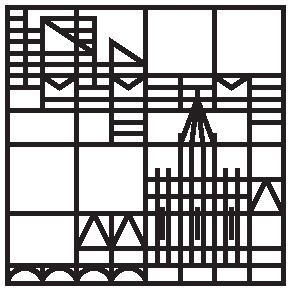
\includegraphics[width=5cm]{logo}
\\ \Large Universität Konstanz  \\ \vspace{4ex} \huge 
Skript zur Vorlesung\\ Höhere Quantentheorie und Elektrodynamik
\\ \vspace{4ex} \Large Prof. Dr. Wolfgang Belzig 
\\ Version vom 30. Juli 2012 \\ \vspace{4.5cm}
\normalsize Ursprünglichen Mitschrift von Birte Heinze im WS 09/10 \\ Ausführliche Überarbeitung von Tobias Lohse im WS 11/12 \vspace{-10cm}}
\author{}
\date{}
%\begin{document}

\subsection{Addition von Drehimpulsen}

In manchen Systemen ist der Gesamtdrehimpuls, welcher als Summe aus Bahndrehimpuls und Spin oder Summe aus den Spins oder Gesamtdrehimpulsen mehrerer Teilchen definiert ist, eine wichtige Größe. Es ist daher hilfreich die Addition von zwei allgemeinen Drehimpulsoperatoren $\hat{\vec{J}}_1$ und $\hat{\vec{J}}_2$ näher zu untersuchen. Der {\bf Gesamtdrehimpuls} $\hat{\vec{J}}$ ist gegeben durch: 
\begin{eqnarray*}
\hat{\vec{J}} &=& \hat{\vec{J}}_1+\hat{\vec{J}}_2
\end{eqnarray*}
Die Drehimpulsoperatoren $\hat{\vec{J}}_1$ und $\hat{\vec{J}}_2$ erfüllen die Drehimpulsalgebra (\ref{Drehimpulsalgebra}) und vertauschen Komponentenweise untereinander aber nicht mit dem Gesamtdrehimpulsquadrat $\hat{J}^2$: 
\begin{eqnarray*}
	\big[\hat{J}_{1i},\hat{J}_{2j}\big] &=& 0 \qquad \forall i\neq j \qquad i,j\in\{x,y,z\}
	\\
	\big[\hat{J}_{1/2\;i},\hat{J}^2\big] &\neq& 0 \qquad \forall i\neq j \qquad \text{mit: } \hat{J}^2=\hat{J}_1^2+\hat{J}_2^2+2\cdot\hat{\vec{J}}_1\cdot\hat{\vec{J}}_2
\end{eqnarray*}
Dies bedeutet, dass wir zwar eine orthonormale Basis mit Produktzuständen $\ket{j_1,m_1}_{\hil_1}\;\oplus\\\ket{j_2,m_2}_{\hil_2}=\;\ket{j_1,j_2,m_1,m_2}_{\hil_1\oplus\hil_2}$ der beiden Drehimpulsoperatoren $\hat{\vec{J}}_1$ und $\hat{\vec{J}}_2$ finden, diese allerdings nicht orthogonal zu den Eigenzuständen des Gesamtdrehimpulses $\ket{j,m}$ sind. 

Dieser Umstand ist relevant für die Erklärung, der Spin-Bahn-Kopplung in Atomen (welche sich allerdings nur mittels relativistischer Quantenmechanik erklären lässt) und der Bandstruktur von Festkörpern und damit insbesondere Halbleitern. 


\subsubsection{Addition von zwei Spin 1/2-Operatoren}

Wir wollen die Addition von Drehimpulsen zunächst am Beispiel zweier Spin 1/2-Operatoren $\hat{\vec{S}}_1$ und $\hat{\vec{S}}_2$ untersuchen. Diese beiden Operatoren sollen wie gesagt komponentenweise miteinander vertauschen und die Drehimplusalgebra erfüllen. Die möglichen Zustände der beiden Teilsysteme $\ket{s_i,m_i}$ sind dann wie wir wissen $s = 1/2$ und $m = \pm 1/2$, die beiden Teilhilberträume $\hil_i$ sind also nur zweidiagonal. Wir führen die übliche abkürzende Schreibweise für die beiden Basiszustände ein: 
\begin{eqnarray*}
	\ket{1/2,+1/2} &=:& \up \qquad\text{wird als 'spin up' bezeichnet}
	\\
	\ket{1/2,-1/2} &=:& \down \qquad\text{wird als 'spin down' bezeichnet}
\end{eqnarray*}
Der Produktraum der beiden Spin-Systeme besitzt dann die vier folgenden Basiszustände:
\begin{eqnarray*}
	\up_{\hil_1}\;\oplus\up_{\hil_2} =\;\upup &\qquad& \down_{\hil_1}\;\oplus\down_{\hil_2} =\;\downdown
	\\
	\up_{\hil_1}\;\oplus\down_{\hil_2} =\;\updown &\qquad& \down_{\hil_1}\;\oplus\up_{\hil_2} =\;\downup
\end{eqnarray*}
Im folgenden werden wir Planck-Einheiten verwenden, also $\hbar=1$ setzen. Der Gesamtspin $\hat{\vec{S}}=\hat{\vec{S}}_1 + \hat{\vec{S}}_2$ erfüllt ebenfalls die Drehimpulsalgebra und seine Eigenzustände haben damit auch die Form $\ket{s,m}$. Wobei die Quantenzahl $m$ den Gesamtdrehimpuls in $z$-Richtung angibt: $\hat{S}_z = \hat{S}_{1z} + \hat{S}_{2z}$. Es sollen also nun die möglichen Werte für $s$ und $m$ bestimmt werden. Dazu untersuchen wir zunächst die Wirkung des Operators $\hat{S}_z$ auf die Basiszustände $\ket{s_1,m_1,s_2,m_2}=\ket{\uparrow\!\!/\!\!\downarrow\;\uparrow\!\!/\!\!\downarrow}$: 
\begin{eqnarray*}
	\hat{S}_z \upup = (\hat{S}_{1z} + \hat{S}_{2z})\upup = \Big(\frac12+\frac12\Big)\upup &=& +1\cdot\upup
	\\
	\hat{S}_z \updown/\downup = \Big(\pm\frac12\mp\frac12\Big)\updown/\downup &=& 0\cdot\updown/\downup
	\\
	\hat{S}_z \downdown = \Big(-\frac12-\frac12\Big)\downdown &=& -1\cdot\downdown 
\end{eqnarray*}
Die Werte von $m$ sind somit ganzzahlig und nehmen werte zwischen $-1$ und $+1$ an.

Nun wollen wir die Werte für $s$ bestimmen, indem wir die Wirkung des Opeators $\hat{\vec{S}}^{\;2}$ untersuchen. Diesen schreiben wir dazu zunächst wie folgt: 
\begin{eqnarray*}
	\hat{S}^2 &=& \hat{S}_1^2 + \hat{S}_2^2 + 2\cdot\hat{\vec{S}}_1\cdot\hat{\vec{S}}_2 = \hat{S}_1^2 + \hat{S}_2^2 + 2\hat{S}_{1z}\hat{S}_{2z} +2 \hat{S}_{1x} \hat{S}_{2x} + 2\hat{S}_{1y}\hat{S}_{2y} 
	\\
	&=& \hat{S}_1^2 + \hat{S}_2^2 + 2\hat{S}_{1z}\hat{S}_{2z}+S^{+}_1S^{-}_2 + S^{-}_1 S^+_2
\end{eqnarray*}
Für den Spin 1/2 gilt nun $\hat{S}_{1/2}^2\up/\down = 1/2\cdot(1/2+1) \up/\down = 3/4 \up/\down$. Und somit ergibt sich für die Wirkung des Operators $\hat{S}^2$ auf den Zustand $\upup$ folgendes: 
\begin{eqnarray*}
	&& \hat{S}^2 \upup = \Big(\frac34+\frac34+2\cdot\frac12\cdot\frac12+0+0\Big) \upup = 2\cdot \upup = 1\cdot(1+1) \upup \;\overset!=\; s(s+1) \upup 
	\\
	&\Rightarrow& \upup \;=\; \ket{s=1,m=1}
\end{eqnarray*}
Auf die selbe Weise können wir den Zustand $\downdown$ als $\ket{s=1,m=-1}$ identifizieren. 
 
Um den Zustand $\ket{s=1,m=0}$ zu bestimmen, verwenden wir den Operator $\hat{S}^-=\hat{S}_1^-+\hat{S}_2^-$, dessen Wirkung auf $\ket{s,m}$ wir kennen: $\hat{S}^-\ket{s,m}=\sqrt{s(s+1)-m(m-1)}\ket{s,m-1}$. Somit ergibt sich: 
\begin{eqnarray*}
	&&\hat{S}^-\upup = (\hat{S}_1^-+\hat{S}_2^-)\upup = \downup+\updown \quad=\quad \hat{S}^-\ket{1,1} = \sqrt2 \ket{1,0}
	\\
	&\Rightarrow& \ket{1,0} \;=\; \frac1{\sqrt2}\cdot(\updown+\downup)
\end{eqnarray*}
Der letzte Basiszustand $\ket{s=0,m=0}$ ergibt sich unter Ausnutzung der Orthogonalitäts-Bedingung dann als $1/\sqrt2\cdot(\updown-\downup)$. 

Die Eigenzustände von $\hat{S}^2$ und $\hat{S}_z$ werden abhängig vom Wert der Gesamtspinquantenzahl in zwei Gruppen eingeteilt: 
\begin{itemize1}
	\item Den sogenannten {\bf Singulet} Zustand: 
	\\$\ket{0,0}=1/\sqrt2\cdot(\updown-\downup)$
	\item Und die sogenannten {\bf Triplet} Zustände: 
	\\$\ket{1,0}=1/\sqrt2\cdot(\updown-\downup)$
	\\$\ket{1,1}=\upup$
	\\$\ket{1,-1}=\downdown$
\end{itemize1}



\subsubsection{Addition von zwei allgemeinen Drehimpulsoperatoren}

Wir wollen nun den Fall zweier allgemeiner Drehimpulsoperatoren $\hat{\vec{J}}_1$ und $\hat{\vec{J}}_2$ betrachten. Diese vertauschen wie bereits beschrieben Komponentenweise untereinander und erfüllen die Drehimpulsalgebra. Wir werden auch hier im folgenden Planck-Einheiten $\hbar=1$ verwenden. 

In einen Raum indem ein Drehimpulsoperator definiert werden kann, lässt sich für den Teilraum, welcher die Drehimpulssymmetrie beschreibt, eine vollständige orthonormale Basis immer in Eigenzuständen des Operators des Drehimpulsbetrags $\hat{J}_i^2\ket{j_i,m_i}=j_i(j_i+1)\ket{j_i,m_i}$ und des Operators des Drehimpluses in $z$-Richtung $\hat{J}_{iz}\ket{j_i,m_i}=m_i\ket{j_i,m_i}$ beschreiben. Als Basis des Produktraums, indem beide Drehimpulsoperatoren definiert sind, können wir dann folgende Zustände wählen: $\ket{j_1,m_1}_{\hil_1}\;\oplus\ket{j_2,m_2}_{\hil_2}=\ket{j_1,j_2,m_1,m_2}$. 

Der Gesamtdrehimpuls ergibt sich aus der Addition der beiden Drehimpulse $\hat{\vec{J}}=\hat{\vec{J}}_1+\hat{\vec{J}}_2$ und erfüllt damit ebenso die Drehimpulsalgebra (\ref{Drehimpulsalgebra}). Damit gibt es eine weitere Basis mit Eigenzuständen des Operators des Gesamtdrehimpulsbetrags $\hat{J}^2\ket{j,m}=j(j+1)\ket{j,m}$ und des Operators des Gesamtdrehimpulses in $z$-Richtung $\hat{J}_z\ket{j,m}=m\ket{j,m}$. Da der Gesamtdrehimpulsbetrag mit den einzelnen Drehimpulsbeträgen vertauscht $[\hat{J}^2,\hat{J}_{1/2}^2]=0$, ist eine weitere vollständige orthonormale Basis des Systems durch die Zustände $\ket{j_1,j_2,j,m}$ gegeben. 

Da der Operator des Gesamtdrehimpulsbetrags jedoch nicht mit den Operatoren der einzelnen Drehimpulse in $z$-Richtung vertauscht, sind die Basiszustände $\ket{j_1,j_2,m_1,m_2}$ und $\ket{j_1,j_2,j,m}$ nicht identisch. Wir suchen daher die Koordinaten der Eigenzustände der letzteren Darstellung in der ersten Darstellung: 
\begin{eqnarray*}
	\ket{j_1,j_2,j,m} = \sum_{m_1,m_2} \underbrace{\braket{j_1,j_2,m_1,m_2}{j_1,j_2,j,m}}_{=C_{m_1,m_2}^{j,m}}\cdot \ket{j_1,j_2,m_1,m_2} 
\end{eqnarray*}
Es muss hier nicht über $j_1$ und $j_2$ summiert werden, da die Zustände in beiden Basen Eigenzustände von $\hat{J}_1^2$ und $\hat{J}_2^2$ sind und die Eigenzustände zu verschiedenen Eigenwerten $j_1$ oder $j_2$ somit orthogonal sind. Manchmal werden die Zustände daher auch etwas unvollständig als $\ket{m_1,m_2}$ und $\ket{j,m}$ geschrieben. Außerdem ist die Summe beschränket auf alle Kombinationen von $m_1$ und $m_2$ für die gilt: $m_1+m_2=m$. Dies lässt sich leicht einsehen, wenn man die Eigenzustände des Gesamtdrehimpulsoperators in $z$-Richtung $\hat{J}_z=\hat{J}_{1z}+\hat{J}_{2z}$ betrachtet, welche sich wie man leicht sieht als $m=m_1+m_2$ ergeben. Die Koordinaten $C_{m_1,m_2}^{j,m}$ werden als {\bf Clebsch-Gordan-Koeffizienten} bezeichnet und sind für verschiedenste Systeme tabelliert. 

Folgendes ist dabei über die Zustände anzumerken: 
\begin{itemize1}
	\item Die Gesamtdrehimpuls-Quantenzahl $j$ ist bei gegebenen $j_1$ und $j_2$ auf folgende Werte beschränkt: $|j_1-j_2|\leq j \leq |j_1 + j_2|$. 
	\item Die Anzahl der Zustände im $j_1$-$j_2$ Unterraum für einen festen Wert von $j_1$ und $j_2$ und die üblichen $2j_i+1$ Zuständen pro $j_i$ lässt sich für $j_1\geq j_2$ bestimmen zu: 
	\begin{eqnarray*}
	\dim\big(\hil_{j_1,j_2}\big) = \sum_{j=|j_1-j_2|}^{|j_1+j_2|} 2j+1 \overset{(k=j-j_1)}= \sum_{k =-j_2}^{+j_2} 2\cdot(j_1 + k)+1 &=& (2j_1 +1)\cdot(2j_2+1)
	\end{eqnarray*}
\end{itemize1}

\paragraph{Systhematische Vorgehensweise zur Bestimmung der Clebsch-Gordan-Koeffizienten}

Im folgenden soll ein systematisches Verfahren zur Bestimmung der Clebsch-Gordan-Koeffizienten $C_{m_1,m_2}^{j,m}$ für zwei beliebige Drehimpulsoperatoren beschrieben werden. Wir benutzen dazu die oben beschriebene Notation, wobei wir die Zustände verkürzt als $\ket{j,m}$ und $\ket{m_1,m_2}$ beschreiben. 

\begin{itemize1}
	\item Zunächst können wir einen Ausgangszustand völlig frei wählen, konventionell ist dies der Zustand mit maximalem Gesamtdrehimpuls $\ket{j=j_1+j_2,m=j_1+j_2}:=\ket{m_1=j_1,m_2=j_2}$, wir legen also $C_{j_1,j_2}^{j_1+j_2,j_1+j_2}=1$ fest. 
	\item Der zweite Schritt besteht darin Zustände mit demselben Gesamtdrehimpulsbetrag aber anderem Gesamtdrehimpuls in $z$-Richtung zu erzeugen. Dazu wenden wir den Leiteroperator $\hat{J}^-=\hat{J}^-_1+\hat{J}^-_2$ auf die Zustände in beiden Notationen an: 
	\begin{eqnarray*}
		\hat{J}^- \ket{j,m} &=& a^-_{j,m} \ket{j,m-1} \quad =
		\\ 
		(\hat{J}^-_1+\hat{J}^-_2) \ket{m_1,m_2} &=& a^-_{j_1,m_1}\ket{m_1-1,m_2} + a^-_{j_2,m_2}\ket{m_1,m_2-1}
	\end{eqnarray*}
	Wobei die Koeffizienten gegeben sind  durch: $a^-_{j,m}=\sqrt{j(j+1)-m(m-1)}$. Wir können nun die Clebsch-Gordan-Coeffizienten $C^{j,m-1}_{m_1-1,m_2}$ und $C^{j,m-1}_{m_1,m_2-1}$ bestimmen, indem wir die obige Gleichung mit $\bra{m_1-1,m_2}$ beziehungsweise $\bra{m_1,m_2-1}$ multiplizieren. Es ergibt sich dann unter Ausnutzung der Orthogonalität der $\ket{m_1,m_2}$ Zustände folgendes: 
	\begin{eqnarray*}
	C^{j,m-1}_{m_1-1,m_2} = \braket{m_1-1,m_2}{j,m-1} = \frac{a^-_{j_1,m_1}}{a^-_{j,m}} && C^{j,m-1}_{m_1,m_2-1} = \braket{m_1,m_2-1}{j,m-1} = \frac{a^-_{j_2,m_2}}{a^-_{j,m}}
	\end{eqnarray*}
	Ausgehend vom ersten Zustand können somit dann die Koeffizienten $C^{j_1+j_2,j_1+j_2-1}_{j_1-1,j_2}$ und $C^{j_1+j_2,j_1+j_2-1}_{j_1,j_2-1}$ bestimmt werden. 
	\item Im dritten Schritt werden die zu den Zuständen $\ket{j,m}$ orthogonalen Zustände $\ket{j-1,m}$ konstruiert, indem wir die in Schritt zwei hergeleitete Notation benutzen, von der aus man den Orthogonalen Zustand direkt sehen kann: 
	\begin{eqnarray*}
	\ket{j,m-1} &=& C^{j,m-1}_{m_1-1,m_2} \ket{m_1-1,m_2} + C^{j,m-1}_{m_1,m_2-1} \ket{m_1,m_2-1}
	\\
	\Rightarrow\quad \ket{j-1,m-1} &=& C^{j,m-1}_{m_1-1,m_2} \ket{m_1-1,m_2} - C^{j,m-1}_{m_1,m_2-1} \ket{m_1,m_2-1}
	\end{eqnarray*}
	Die Koeffizienten ergeben sich dann zu: $C^{j-1,m-1}_{m_1-1,m_2}=C^{j,m-1}_{m_1-1,m_2}$ und $C^{j-1,m-1}_{m_1,m_2-1}=-C^{j,m-1}_{m_1,m_2-1}$. Ausgehend von den ersten drei Zuständen können dann  Somit beispielsweise die beiden Koeffizienten $C_{j_1-1,j_2}^{j_1+j_2-1,j_1+j_2-1}$ und $C_{j_1,j_2-1}^{j_1+j_2-1,j_1+j_2-1}$ bestimmt werden. 
	\item Nun ist die Quantenzahl $m$ wieder maximal für den neuen Wert von $j-1$ und es kann wiederum Schritt zwei und drei auf die beiden neu entstandenen Zustände angewandt werden und das Verfahren so lange wiederholt werden, bis alle Clebsch-Gordan-Koefizienten bestimmt sind. 
\end{itemize1}

%\end{document}